\section{Anwendung der Integralrechnung}\label{sec:anwendung-der-integralrechnung}

\textbf{Repetition:} Das \emph{bestimmte Integral} einer Funktion $f$ ist wie folgt definiert: \[\int_{a}^{b} f(x) \diff{x} = \lim_{n \rightarrow \infty} \sum_{k=1}^{n} f(x_K) \Delta x\]

\subsection{Mittelwert}\label{subsec:mittelwert}

\begin{center}
    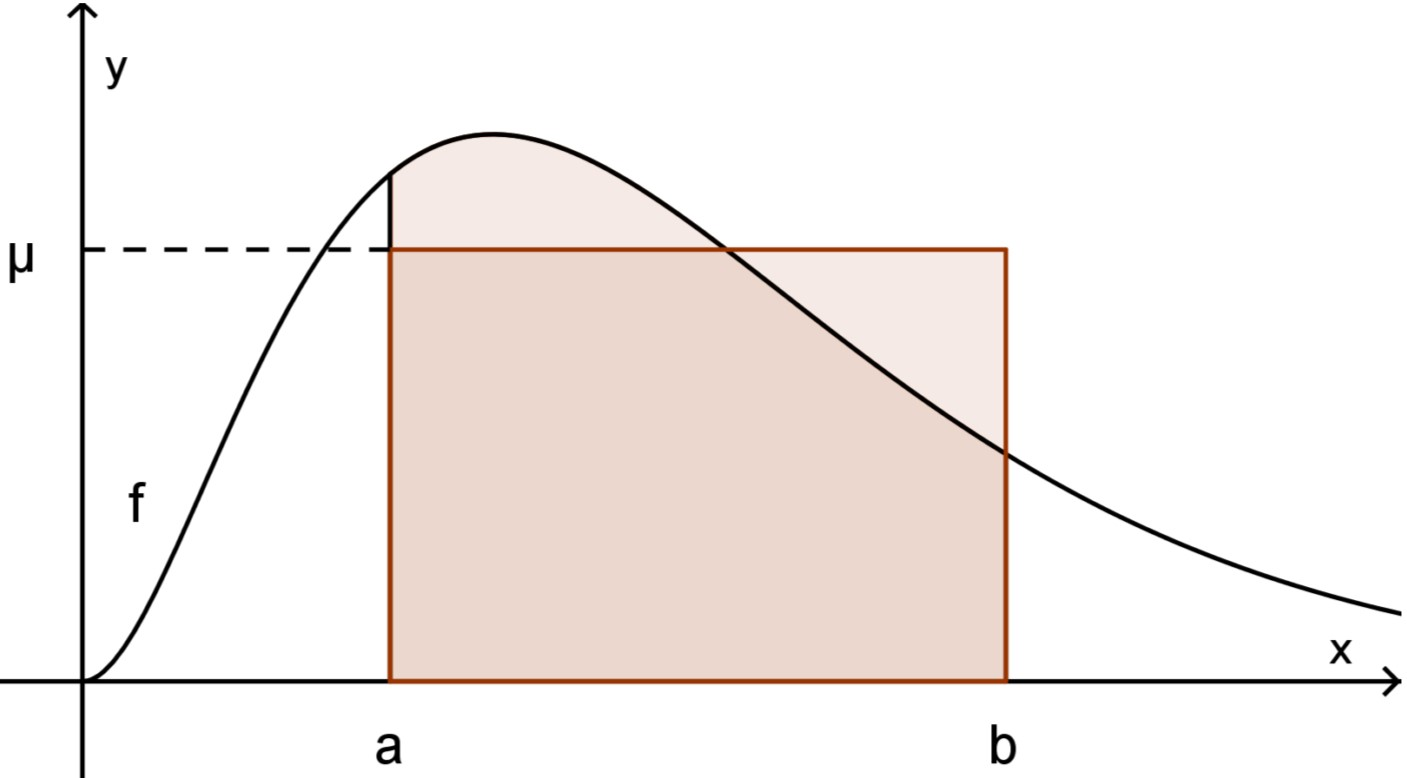
\includegraphics[scale=0.15]{mittelwert}
\end{center}

\begin{definition}{Mittelwert}
    Gegeben ist eine Funktion $f$ mit $f(x) \leq 0$ für alle $x \in [a,b]$.
    Unter dem \emph{Mittelwert} $\mu$ von $f$ versteht man die Höhe jenes Rechtecks,
    \begin{itemize}
        \item das eine Grundlinie der Länge $b - a$ hat, und
        \item dessen Flächeninhalt der Fläche unter der Kurve, resp. $\int_{a}^{b} f(x) \diff{x}$, entspricht.
    \end{itemize}
    Daraus folgt: \[\mu = \frac{1}{b - a} \cdot \int_{a}^{b} f(x) \diff{x}\]
\end{definition}

\textbf{Beispiel:} Berechnen Sie den Mittelwert von $f(x) = x^2 + 2$ auf dem Intervall $[2,4]$.
\begin{align*}
    \mu &= \frac{1}{4 - 2} \cdot \int_{2}^{4} (x^2 + 2) \diff{x} = \frac{1}{2} \cdot \left( \int_{2}^{4} x^2 \diff{x} + \int_{2}^{4} 2 \diff{x} \right) = \frac{1}{2} \cdot \left( \left[ \frac{x^3}{3} \right]_{2}^{4} + \left[ 2x \right]_{2}^4 \right) \\
    &= \frac{1}{2} \cdot \left( \frac{4^3}{3} - \frac{2^3}{3} + (8 - 4) \right) = \frac{34}{3}
\end{align*}

\subsection{Volumen eines Rotationskörpers}\label{subsec:volumen-eines-rotationskorpers}

\begin{definition}{Volumen eines Rotationskörpers (Drehung um $x$-Achse)}
    Gegeben ist eine Funktion $f$ mit $f(x) \leq 0$ für alle $x \in [a,b]$.
    Dreht man das Flächenstück um die $x$-Achse, so entsteht ein \emph{Rotationskörper} mit dem folgenden Volumen: \[V = \pi \cdot \int_{a}^{b} (f(x))^2 \diff{x}\]
\end{definition}

\begin{center}
    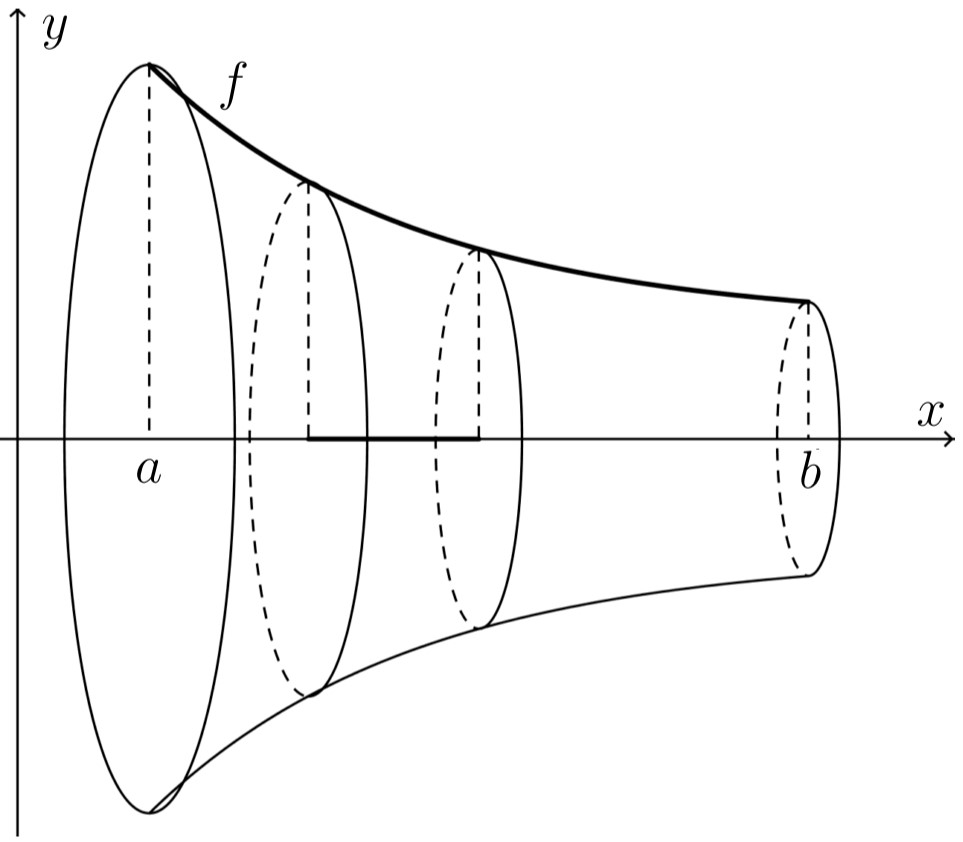
\includegraphics[scale=0.25]{volumen-rotationskoerper}
\end{center}

\textbf{Beispiel:} $f(x) = x^2 + 1$, $a = -1$, $b = 1$.
Berechnen Sie das Volumen des entsprechenden Rotationskörpers.
\begin{align*}
    V &= \pi \int_{-1}^{1} (x^2 + 1)^2 \diff{x} = \pi \int_{-1}^{1} x^4 + 2 x^2 + 1 \diff{x} = \pi \left( \int_{-1}^{1} x^4 \diff{x} + 2 \int_{-1}^{1} x^2 \diff{x} + \int_{-1}^{1} 1 \diff{x} \right) \\
    &= \pi \left( \left[ \frac{x^5}{5} \right]_{-1}^{1} + 2 \left[ \frac{x^3}{3} \right]_{-1}^{1} + [x]_{-1}^{1} \right) = \pi \left( \frac{1}{5} - \left( -\frac{1}{5} \right) + 2 \cdot \left( \frac{1}{3} - \left( -\frac{1}{3} \right) \right) + 1 - (-1) \right) = \frac{56}{15} \pi
\end{align*}

\begin{definition}{Volumen eines Rotationskörpers (Drehung um $y$-Achse)}
    Gegeben ist eine Funktion $y = f(x)$ mit $x \leq 0$ für alle $y \in [c, d]$.
    Dreht man das Flächenstück, das zwischen dem Graphen von $f$, der $y$-Achse und den beiden Grenzen $y = c$ und $y = d$ liegt, \textbf{um die $y$-Achse}, so entsteht ein Rotationskörper mit den folgenden Volumen: \[V = \pi \cdot \int_{c}^{d} (g(y))^2 \diff{y}\] wobei $g(y)$ die nach $x$ aufgelöste Funktionsgleichung ist.
\end{definition}

\begin{center}
    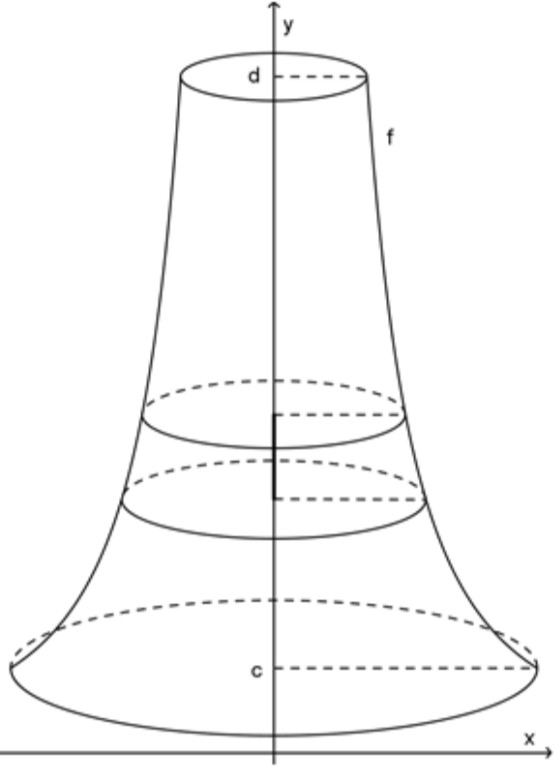
\includegraphics[scale=0.25]{volumen-rotationskoerper-y-achse}
\end{center}

\textbf{Beispiel:} Das Kurvenstück $y = \sqrt {x}$ wird im Intervall $0 \geq y \geq 5$ um die $y$-Achse rotiert.
Wie gross ist das Volumen des entsprechenden Rotationskörpers?

$y = \sqrt {x}$ \\
Umkehrfunktion: $y^2 = x \Rightarrow g(y) = y^2$

$\Rightarrow V = \pi \int_{0}^{5} (y^2)^2 \diff{y} = \pi \int_{0}^{5} y^4 \diff{y} = \pi \cdot \left[ \frac{y^5}{5} \right]_{0}^{5} = \pi \cdot \frac{5^5}{5} = 625 \pi$

\subsection{Bogenlänge einer ebenen Kurve}\label{subsec:bogenlange-einer-ebenen-kurve}

\begin{definition}{Bogenlänge einer ebenen Kurve}
    Wir betrachten eine Funktion $y = f(x)$ über einem Intervall $[a,b]$.
    Die Bogenlänge dieser Kurve beträgt \[s = \int_{a}^{b} \sqrt {1 + (y')^2} \diff{x}\]
\end{definition}

\begin{center}
    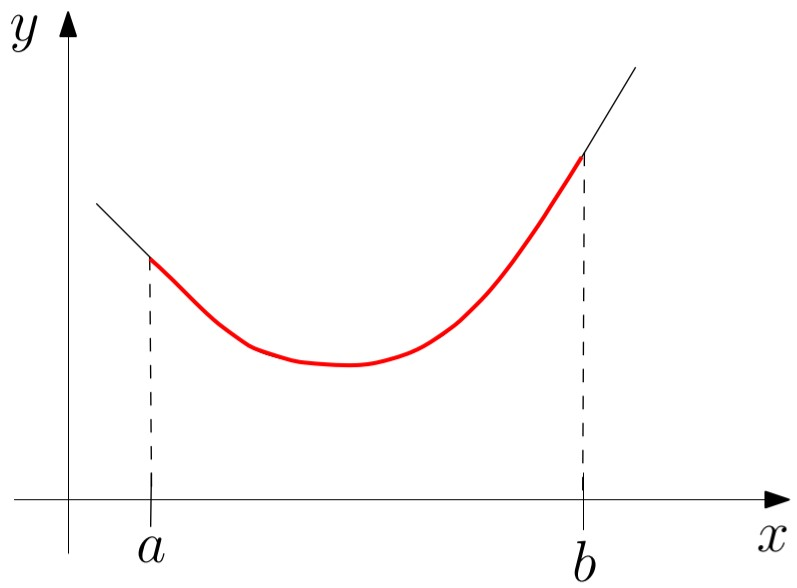
\includegraphics[scale=0.25]{bogenlaenge}
\end{center}

\newpage

\subsection{Mantelfläche eines Rotationskörpers}\label{subsec:mantelflache-eines-rotationskorpers}

\begin{definition}{Mantelfläche eines Rotationskörpers}
    Die \emph{Mantelfläche} bezeichnet die Oberfläche eines Körpers ohne seinen Deckel und Boden.
    Wir betrachten eine Funktion $y = f(x)$ mit $f(x) \leq 0$ für alle $x \in [a,b]$.
    Dreht man das Flächenstück, das im Intervall $[a,b]$ zwischen dem Graphen von $f$ und der $x$-Achse liegt, um die $x$-Achse, so entsteht ein Rotationskörper mit der folgenden Mantelfläche: \[M = 2 \pi \cdot \int_{a}^{b} y \cdot \sqrt {1 + (y')^2} \diff{x}\]
\end{definition}

\textbf{Beispiel:}

Das Kurvenstück $y = \sqrt{x}$ wird im Intervall $0 \geq x \geq 2$ um die $x$-Achse rotiert.
Berechnen Sie die Mantelfläche des entstehenden \emph{Paraboloids}.

$y = \sqrt{x} = x^{1/2}$, $y' = \frac{1}{2} x^{-1/2)}$, $1 + (y')^2 = 1 + \frac{1}{4x}$

$M = 2 \pi \int_{0}^{2} \sqrt{x} \cdot \sqrt {1 + \frac{1}{4x}} \diff{x} = 2 \pi \int_{0}^{2} \sqrt {x + \frac{1}{4}} \diff{x} = 2 \pi \cdot \left[ \frac{2}{3} \left( x + \frac{1}{4} \right)^{3/2} \right]_{0}^{2} = \frac{13 \pi}{3} \approx 13.61$

\subsection{Schwerpunkt}\label{subsec:schwerpunkt}

\begin{definition}{Bedeutung Schwerpunkt (Physik)}
    Ein fester Körper verhält sich häufig so, als wäre seine gesamte Masse in seinem \emph{Schwerpunkt} vereinigt.
    Diese ist sozusagen das gewichtete Mittel aller Massenpunkte.
\end{definition}

\begin{definition}{Schwerpunkt einer Fläche zwischen zwei Kurven}
    \begin{multicols}{2}
        Der Schwerpunkt des Flächenstücks, das im Intervall $[a,b]$ zwischen den Graphen von $f_o(x)$ und $f_u(x)$ liegt, hat die Koordinaten:
        \begin{align*}
            &x_s = \frac{1}{A} \int_{a}^{b} x \cdot (f_o(x) - f_u(x)) \diff{x} \\
            &y_s = \frac{1}{2A} \int_{a}^{b} (f_o^2(x) - f_u^2(x)) \diff{x}
        \end{align*}
        \begin{center}
            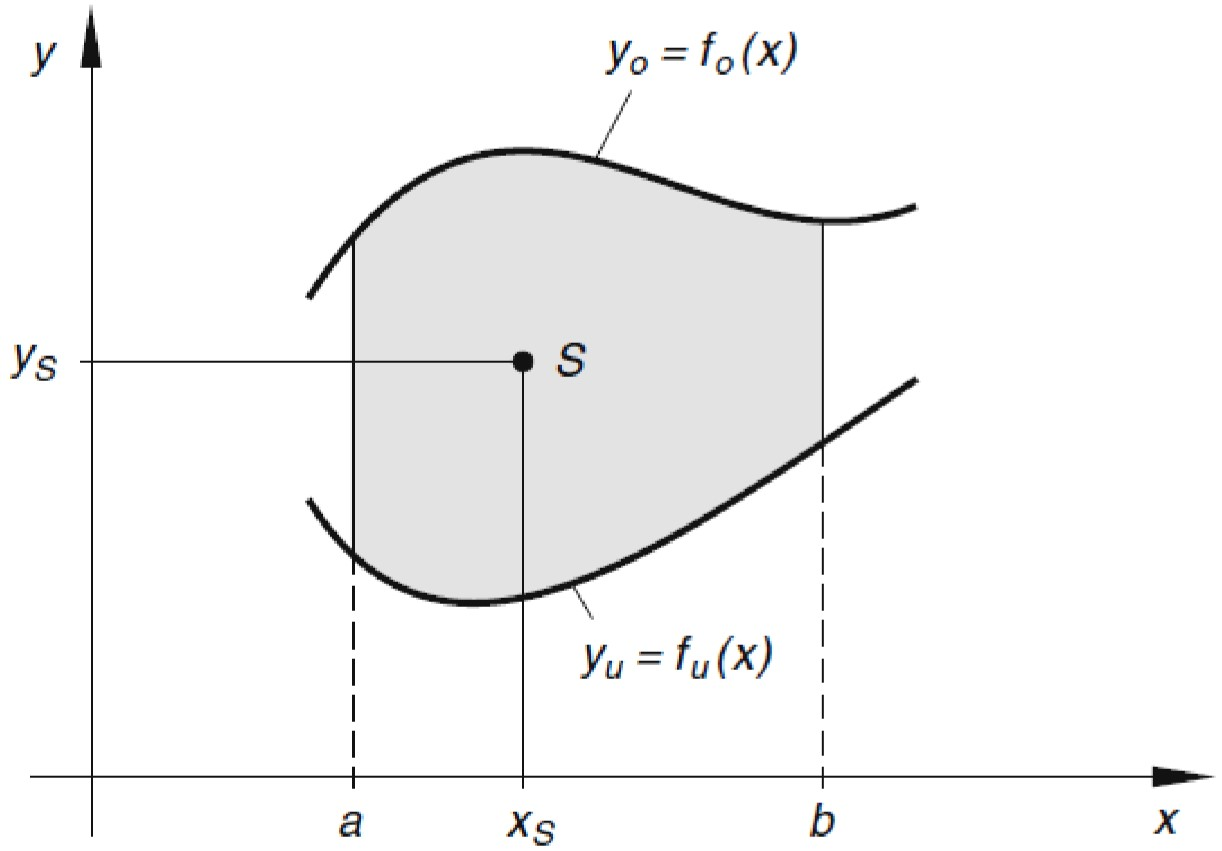
\includegraphics[scale=0.25]{schwerpunkt-flaeche}
        \end{center}
    \end{multicols}
\end{definition}

\begin{definition}{Schwerpunkt eines Rotationskörpers}
    \begin{multicols}{2}
        Wir betrachten eine Funktion $y = f(x)$ mit $f(x) \leq 0$ für alle $x \in [a,b]$.
        Dreht man das Flächenstück, das im Intervall $[a,b]$ zwischen dem Graphen von $f$ und der $x$-Achse liegt, um die $x$-Achse, so entsteht ein Rotationskörper.
        Sein Schwerpunkt hat folgende Koordinaten:
        \[x_s = \frac{\pi}{V} \int_{a}^{b} x \cdot f^2(x) \diff{x} \quad\quad y_s = 0 \quad\quad z_s = 0\]
        \begin{center}
            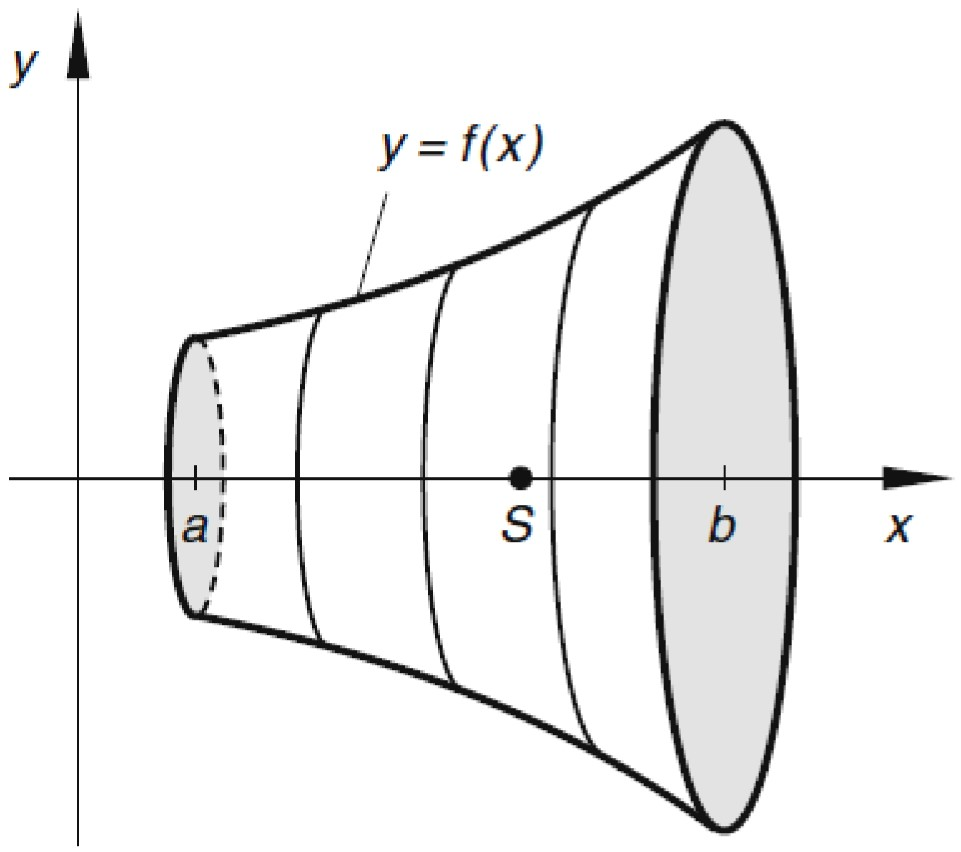
\includegraphics[scale=0.25]{schwerpunkt-koerper}
        \end{center}
    \end{multicols}
\end{definition}